\documentclass[tikz,border=2pt]{standalone}
\usepackage{amsmath}
\usepackage{pgfplots}
\pgfplotsset{compat=1.18}
\usetikzlibrary{arrows.meta}
\begin{document}
% Second-price auction, value 10: payoff against the highest rival bid r is 10-r if the bid
% exceeds r, else 0. Bidding 10 and bidding 8 tie for r<8 and r>10 and bidding 10 is strictly
% better for 8<r<10 (e.g. r=9: 1 versus 0; r=7: 3 and 3; r=12: 0 and 0).
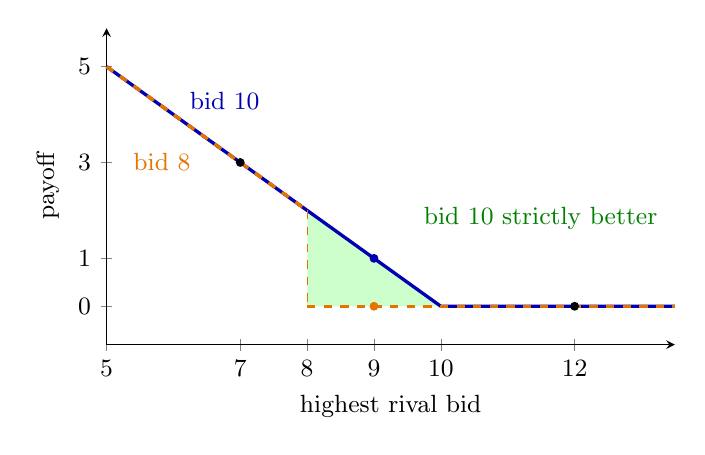
\begin{tikzpicture}[font=\small, >={Latex[length=2mm]}]
  \begin{axis}[width=8.8cm, height=5.6cm, axis lines=left,
      xmin=5, xmax=13.5, ymin=-0.8, ymax=5.8,
      xtick={5,7,8,9,10,12}, ytick={0,1,3,5},
      xlabel={highest rival bid}, ylabel={payoff},
      clip=false]
    % region where bidding 10 is strictly better
    \fill[green!20] (axis cs:8,0) -- (axis cs:8,2) -- (axis cs:10,0) -- cycle;
    % bid 10 (truthful)
    \draw[very thick, blue!70!black] (axis cs:5,5) -- (axis cs:10,0) -- (axis cs:13.5,0);
    % bid 8
    \draw[very thick, orange!90!black, dashed] (axis cs:5,5) -- (axis cs:8,2);
    \draw[very thick, orange!90!black, dashed] (axis cs:8,0) -- (axis cs:13.5,0);
    \draw[thin, orange!90!black, dashed] (axis cs:8,2) -- (axis cs:8,0);
    % checked rival bids
    \fill[black] (axis cs:7,3) circle (1.6pt);
    \fill[blue!70!black] (axis cs:9,1) circle (1.6pt);
    \fill[orange!90!black] (axis cs:9,0) circle (1.6pt);
    \fill[black] (axis cs:12,0) circle (1.6pt);
    \node[blue!70!black, anchor=south west] at (axis cs:6.1,3.9) {bid $10$};
    \node[orange!90!black, anchor=north east] at (axis cs:6.4,3.4) {bid $8$};
    \node[green!50!black, anchor=south west] at (axis cs:9.6,1.4) {bid $10$ strictly better};
  \end{axis}
\end{tikzpicture}
\end{document}
